\chapter{Background}
\label{ch:background}

\section{Chapter Overview}

In this chapter, we review some of the background critical to this dissertation.
We begin with a discussion of Recognizing Textual Entailment (RTE) as core
motivation of our thesis.  We then overview Distributional Semantics, outlining
its purpose and two specific implementations employed in this thesis. Finally,
we discuss the Lexical Entailment (LexEnt) and Lexical Substitution (LexSub)
tasks, which we view as two useful proxies for the kinds of lexical semantics
necessary in RTE. We do not argue that these tasks are completely sufficient,
but one goal of our thesis to show that developments in these tasks improve
practical RTE.

\section{Recognizing Textual Entailment}
\label{sec:textent}

In the previous chapter, we introduced the Recognizing Textual Entailment (RTE)
task as a challenging semantic problem in the field of
Natural Language Processing.  One of the first benchmark papers describes RTE
as ``recognizing, given two text fragments, whether the meaning of one text can
be inferred (entailed) from the other'' \cite{dagan:2006:mlc}. For example,
an RTE system could read the sentence ``A bright girl reads a book,'' and
predict it entails ``A smart child looks at text.''

Since this original definition, many other datasets
\cite{giampiccolo:2007:pascal,bentivogli:2009:tac,marelli:2014:semeval} and
countless approaches have been described (c.f. \newcite{dagan:2013:synthesis}
for a thorough survey). Although RTE is not usually considered an
end-user application by itself, successful RTE systems may influence many
downstream tasks like Information Extraction or Question Answering and become
useful in information-heavy industries like defense, journalism, and science.

RTE is a very difficult task, at least partially due to its generality.  True
entailment reasoning may require a mix of common sense and domain-specific
knowledge; sophisticated logical inference about coreference, scope,
quantifiers and implications; and a substantial ability to judge the importance
and relationships between individual lexical items \cite{dagan:2006:mlc}.
Modern RTE systems do {\em not} attempt
to cover every possible entailment phenomenon, but do strive to make
incremental progress on individual problems with varying approaches. In this
thesis, we focus predominantly on some of the issues of {\em lexical semantics}
necessary for reasoning in RTE systems. Specifically, we consider issues like
lexical relationship detection, where one must classify {\em how} two words are
(or are not) related, and lexical paraphrasing, where one must suggest
alternative words which have the same meaning.

Presently, there exist many approaches of RTE systems. Early systems for RTE
focus heavily on detecting word overlap or alignments between the text and
hypothesis. These systems may focus on looking for word re-use between the
two sentences, or the presence of predictive words in either sentence, like
\lit{not} \cite{dagan:2006:mlc}. Modern, deep learning approaches focus
on learning word and sentence representations from large datasets
\cite{bowman:2015:emnlp,cheng:2016:emnlp,bowman:2016:acl,mou:2016:acl,rocktaschel:2016:iclr,vendrov:2016:iclr}.
These models attempt to learn all RTE entailments and word relationships
implicitly through a large dataset of annotated RTE examples. While they
perform incredibly well statistically, recently it has been noted that these
systems boil down to sophisticated variations of the word alignment idea
\cite{parikh:2016:emnlp}, and sometimes fail to learn basic properties about
lexical meaning \cite{pavlick:2016:acl}, and therefore may fail unpredictably,
especially with unseen words.

Other kinds of RTE approaches focus more heavily on doing sorts of logical,
deductive reasoning correctly, but depend heavily on large lexical resources to
capture the implications and information necessary for lexical reasoning
\cite{maccartney:2008:coling,bjerva:2014:semeval,beltagy:2016:cl}. These rich
lexical resources, including WordNet \cite{miller:1995:acm} and PPDB
\cite{ganitkevitch:2013:naacl}, provide an excellent source of common sense
knowledge and word relationships which can be used as a background
knowledge-base during logical reasoning. However, when a word exists outside
the knowledge-base, or the relationship between two words is not labeled, then
the systems will also fail to draw even simple conclusions; as such these
systems may have very high precision, at the extreme cost of recall.

In our work, we consider whether it is possible to improve upon this latter
class of RTE systems by distilling information about lexical relationships
automatically. We turn now to Distributional Semantics and Vector Space Models,
which provide an automatic induction of word meaning using only large,
unannotated corpora.

\section{Distributional Semantics}
\label{sec:dist}

Distributional Semantics is a powerful tool for automatically inducing semantic
representations for lexical items \cite{turney:2010:jair,erk:2012:llc}.  The
core notion is that of the {\em Distributional Hypothesis}, that if two words
appear in similar {\em contexts}, they can be assumed to have similar meaning.
This idea has a long history in the linguistic and philosophical literature that
can be traced back over 60 years
\cite{wittgenstein:1953:pi,harris:1954:word,firth:1957:la}. In its modern form,
Distributional Semantics involves finding {\em vector space representations} of
words which are constructed by counting or modeling the contexts in which a
particular word appears. According to the Distributional Hypothesis, words
with similar {\em vectors} can be assumed to have similar {\em meanings}
\cite{turney:2010:jair}. For this reason, they are often referred to as
Vector Space Models (VSMs) of language. Variations on this idea have also
become immensely popular in the neural networks community, with algorithms
like Skip-gram Negative Sampling (SGNS) \cite{mikolov:2013:iclr} and GloVe
\cite{pennington:2014:emnlp}, and have often replaced traditional count-based
VSMs in the NLP community \cite{baroni:2014:acl}. In their neural forms,
these distributional vectors are often referred to as {\em word embeddings},
because they {\em embed} the word in a fixed-dimensional vector space. In this
dissertation, we freely use the terms {\em embeddings} and {\em word vectors}
interchangeably, and we will cover the SGNS algorithm in more detail in
Section~\ref{sec:word2vec}.

\begin{figure}
\centering
\begin{minipage}{7cm}
\centering
\begin{scriptsize}
\begin{alltt}
         the furry {\color{Cerulean}{dog}} is friendly to    
and manipulate the {\color{Cerulean}{dog}} 's lips and       
       as a clever {\color{Cerulean}{dog}} ; two to          
a reputation among {\color{Cerulean}{dog}} trainers of having
    also among the {\color{Cerulean}{dog}} breeds most likely
 the very earliest {\color{Cerulean}{dog}} shows and kennel  
        as a guard {\color{Cerulean}{dog}} and to hunt       
   the mechanic 's {\color{Cerulean}{dog}} began to howl     
\end{alltt}
\end{scriptsize}~\\
(a) toy corpus
\end{minipage}
\quad
\begin{minipage}{6cm}
\centering
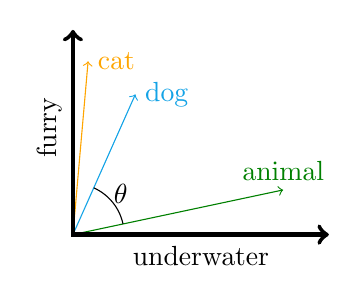
\begin{tikzpicture}[scale=1.3]
    \coordinate (origin) at (0,0);
    \coordinate (cat) at (85:1.7);
    \coordinate (dog) at (66:1.5);
    \coordinate (animal) at (12:2.1);

    \draw [->,Cerulean] (origin) -- (dog) node[right] {\word{dog}};
    \draw [->,Orange] (origin) -- (cat) node[right] {\word{cat}};
    \draw [->,Green] (origin) -- (animal) node[above] {\word{animal}};

    \draw [] (12:0.5) arc (12:66:0.5) node[right,pos=0.75] {$\theta$};
    \draw [<->,ultra thick](2.5,0) -- (origin)  node (yaxis) [below,pos=0.5] {{underwater}}
      -- (0,2.0) node (xaxis) [above,pos=0.5,rotate=90] {{ furry}};
\end{tikzpicture}\\
(b) cartoon vector space
\end{minipage}
\caption{(a) Example contexts of the word \lit{dog}, and (b) cartoon drawing
of word vectors in the \ctx{furry} and \ctx{underwater} dimensions.}
\label{fig:vsm}
\end{figure}

In its simplest form, vectors are induced by defining a vector space where
each dimension in the space corresponds to a particular context word. A large,
unannotated corpus of text is then processed, finding instances of a target word,
like \lit{dog}, and incrementing a count for each of the target's {\em
co-occurrences}, or words appearing around the target word
\lit{dog}, as in Figure~\ref{fig:vsm}. With a large enough corpus, coherent
statistical patterns begin to form. For example, the word \ctx{furry} is likely
to be used to describe both \lit{cat} and \lit{dog}, which is then reflected in
the vector counts \cite{lund:1996:brmic}. After constructing vector
representations for the words \lit{cat} and \lit{dog}, we can then compare
these vectors using various geometric distance metrics, most prominently {\em
cosine similarity}:
\begin{equation}
  \text{cos}(\vu, \vv) = \frac{\sum_i u_iv_i}{\sqrt{\sum_i u_i^2}\sqrt{\sum_i v_i^2}} = \frac{{\vu}^\top{\vv}}{\norm{\vu} \norm{\vv}}
  \label{eqn:cos}
\end{equation}
Here, $i$ iterates over all the different context dimensions, like \ctx{furry}
or \ctx{kennel}, and cosine similarity is defined over the range $[-1, 1]$ or
$[0, 1]$, depending on the exact distributional space chosen.
Words with similar vectors will have a smaller angle between them, and
therefore a higher cosine similarity (i.e. closer to 1). For example, in one of
the distributional spaces used in this thesis, \lit{brother} and \lit{sister}
have a cosine similarity of $0.85$, but \lit{brother} and \lit{truck} have a
cosine similarity of only $0.14$.
% syntactic space used in EMNLP16 paper.
% brother/NN, sister/NN = 0.85
% hot/NN, cold/NN = 0.89

\subsection{Count Transformations}

In practice, usually the distributional vectors are more sophisticated in their
construction than raw co-occurrence counts.  Typically, words and contexts
below a certain threshold are omitted from the co-occurrence matrix, because
extremely rare words have few counts and therefore impoverished representations
\cite{turney:2010:jair}. The co-occurrence matrix is also usually transformed
using some nonlinearity; one common choice is Positive Pointwise Mutual
Information (PPMI) \cite{bullinaria:2007:brm}, where the raw co-occurrence count
between a word $w$ and context $c$ is transformed,
\begin{equation*}
  \text{PPMI}(w, c) = \max\left(0, \log\frac{P(w, c)}{P(w)P(c)}\right)
\end{equation*}
Pointwise Mutual Information (PMI) measures roughly how many times more likely two
items co-occur more often than chance, while Positive PMI
additionally ignores co-occurrences that occur less often than chance.  Other
transformations, like conditional probability ($P(w|c)$ or $P(c|w)$)
\cite{hofman:1999:sigir,blei:2003:jmlr}, Local Mutual Information (LMI)
\cite{evert:2005:phd}, and soft-plus ($\log(1 + x)$)
\cite{pennington:2014:emnlp}, are also sometimes seen in the literature, and
emphasize different aspects of lexical similarity.

\subsection{Context Selection, and Syntactic Contexts}
\label{sec:contextselection}
Defining contexts is another important aspect of distributional semantics.
In the example of Figure~\ref{fig:vsm}, we showed that context can be defined
as three words to the left and right of the target word, but there are
alternatives. For example, using very large windows of co-occurrence (or even
entire documents) results in emphasizing more {\em topical} similarity, e.g. doctor
and hospital, while smaller windows emphasize more {\em functional} similarity, e.g.
doctor and surgeon
\cite{peirsman:2008:essli,agirre:2009:naacl}.

Context can be also defined as {\em syntactic neighbors} extracted from a
dependency parse. For example, in Figure~\ref{fig:syn}, the
contexts for the word {\em chased} would be {\ctx nsubj+dog} and {\ctx
dobj+tail}. Distributional Spaces defined in this manner tend to emphasize the
{\em selectional preferences} of words, or the tendency of words to have
particular arguments in their syntactic relations.
\cite{pado:2007:cl,baroni:2010:cl,levy:2014:acl}. For example,
the subject of {\em barks} is likely to be {\em dog}, while the subject of {\em
purrs} is likely to be {\em cat}.

\begin{figure}
\centering
\begin{dependency}[edge vertical padding=0.5ex, edge style={black},
                   label style={fill=black,text=white,font=\ttfamily}]
  \begin{deptext}[column sep=0.7cm,nodes={font=\Large}]
    the \& dog \& chased \& its \& tail.\\
  \end{deptext}
  \depedge{2}{1}{det}
  \depedge{3}{2}{nsubj}
  \depedge{3}{5}{dobj}
  \depedge{5}{4}{poss}
\end{dependency}
\caption{Example of a dependency parse for ``The dog chased its tail.'' In
a syntactic distributional space, contexts are defined as adjacent nodes
with their labeled edges.}
\label{fig:syn}
\end{figure}

\subsection{Dimensionality Reduction}
Dimensionality Reduction is another important aspect of Distributional Semantics.
As described earlier, distributional vector
spaces are very high-dimensional: bag-of-words spaces have many thousands of
dimensions \cite{turney:2010:jair,mikolov:2013:iclr,pennington:2014:emnlp},
while syntactic spaces may have millions \cite{baroni:2010:cl,pado:2007:cl}.
Efficiently dealing with these large, extremely sparse vectors can be
troublesome, so we often opt to use some form of {\em dimensionality reduction}
in the form of matrix factorization.  In dimensionality reduction, the
co-occurrence matrix $\mM$ is assumed to be factorizable into two lower-rank
matrices,
\begin{equation}
  {\bf M} \approx \mV\mC\trans,
  \label{eqn:factorization}
\end{equation}
where $\mV$ is some lower-rank representation of word vectors, and $\mC$ is
the corresponding lower-rank representation of the context items. These
projections of words and contexts into the same latent space traces back to the
earliest days of distributional semantics
\cite{landauer:1997:pr,deerwester:1990:jsis}, and is critical to many of the
contributions of this thesis.

\paragraph{Singular Value Decomposition}
One common form of matrix factorization used in the literature is the Singular
Value Decomposition. In this formulation, we find a factorization
\begin{equation*}
  \mM = \mA{\bf \Sigma}\mB\trans,
\end{equation*}
where $\mA$ and $\mB$ are unitary matrices, and ${\bf \Sigma}$ is a diagonal
matrix. These three matrices are used to derive the $\mV$ and $\mC$ matrices,
\begin{align*}
  \mV & = \mA{\bf \Sigma},\\
  \mC & = \mB.
\end{align*}
The SVD is particularly important because it is uniquely defined for any
matrix, has a direct connection to the eigendecomposition, and
has natural or domain-specific interpretations. One especially useful property is
that the diagonal matrix ${\bf \Sigma}$ contains an {\em ordered} list of the
{\em singular values} of the matrix. Thus, in its complete form, the ${\bf
\Sigma}$ matrix will actually contain as many entries as the rank of the
matrix, but we arbitrarily pick the first $k$ singular values in order to find
a low-rank approximation \cite{trefethen:1997:linalg}.

\paragraph{Skip-Gram Negative Sampling (Word2Vec)}
\label{sec:word2vec}

More recently, alternative forms of distributional semantics have made a large
impact on the NLP community, in particular the Skip-Gram Negative Sampling
(SGNS) model, commonly known as {\em Word2Vec} \cite{mikolov:2013:iclr}.
Like traditional count-based distributional semantics, SGNS aims to learn a
vector representation for words where words with similar meaning have
similar vectors. It came into wide popularity after the famous observation
that simple vector arithmetic could be used to do some analogical reasoning:
for example, \newcite{mikolov:2013:iclr} famously observed that
\begin{equation*}
  \svec{\text{king}} - \svec{\text{man}} + \svec{\text{woman}} \approx \svec{\text{queen}}.
\end{equation*}

SGNS is a log-bilinear model of co-occurrence, where the model learns {\em
input embeddings} representing words and {\em output embeddings} representing
contexts. These embeddings are $k$-dimensional vectors, typically about $k =
300$, as with other dimensionality reduction models.  The Word2Vec algorithm
learns embeddings in a single pass over a corpus, and does not require storing
any large, sparse co-occurrence matrix, making it much faster and memory
thrifty than traditional count-based models. The algorithm learns by observing
each target word $w$ with a context $c$, just as
Section~\ref{sec:contextselection}. For each co-occurrence observed, the model
pretends that it must perform a classification task, predicting whether the
observed co-occurrence is either real, or random noise according to a
log-bilinear model similar to logistic regression,
\begin{equation}
  P(w|c) = \sigma(\vw\trans\vc),
\end{equation}
where $\sigma$ is the logistic function,
\begin{equation}
  \sigma(x) = \frac{1}{1 + e^{-x}}.
\end{equation}
To turn this it a real classification problem, for each real observed word $w$,
several {\em negative samples} are also ``observed,'' by stochastically selecting
several words $\bar w_1,\ldots,\bar w_n$ from the unigram distribution. The
model should then predict a high probability for the true observation $P(w|c)$
and low probabilities for $P(\bar w_i|c), i = 1,\ldots,n$. In each observation,
the parameters $\vw$ and $\vc$ are updated via Stochastic Gradient Descent
(SGD). With a large corpus, many iterations of SGD are run, resulting in
high-quality representations for $\vw$ and $\vc$.

Initially, the community was perplexed as to why representations learned by
this algorithm should be so much better than those from traditional count-based
methods \cite{baroni:2014:acl}. However, almost all of its mysteries have since
been explained: the SGNS model itself is implicitly equivalent to PMI matrix
factorization \cite{levy:2014:nips}; its improvements over count-based models
are mostly due to heuristics \cite{levy:2015:tacl}; and its analogical
reasoning is related to a balance of cosine similarities
\cite{levy:2014b:conll}. Nonetheless, today the model is often the typical
``default'' choice of NLP practitioners, due to its extreme efficiency and
strong efficacy.

\subsection{Problems with Distributional Representations}

The Distributional Hypothesis and its computational implementations have proven
to be extremely useful in practical applications of NLP \cite{cho:2015:arxiv,goldberg:2016:jair}. Indeed,
one may even argue that the most important and impressive advancements of
the past several years are fundamentally powered through the distributional
hypothesis \cite{manning:2015:cl}. Nonetheless, distributional models do have
a important limitations.

Recall above we showed that the cosine similarity of \lit{brother} and
\lit{sister} is $0.85$, while \lit{brother} and \lit{truck} was only 0.14.
However,  the words \lit{hot} and \lit{cold} have a similarity of $0.89$, even
more than that of \lit{brother} and \lit{sister}. Though the meanings of
\lit{hot} and \lit{cold} are highly related, they are natural antonyms, and it
is (generally) impossible for something to be both hot and cold simultaneously.
Thus we can tell that words have related meanings, but not {\em how} or {\em
why} they are related, or {\em what} is the relationship between them.
Additionally, many measures of distributional similarity, like cosine similarity,
are inherently symmetric, or that
\begin{equation*}
  \text{cos}(\vu, \vv) = \text{cos}(\vv, \vu),
\end{equation*}
thus it is impossible to detect any asymmetric relationship using only cosine
similarity. In the next section, we explore some of these relationships, and
will address these problems in greater detail throughout the thesis.

\section{Lexical Entailment and Relationship Detection}

\newcite{zhitomirskygeffet:2005:acl} define Lexical Entailment as any instance
where one word ``can be substitued by [another word], such that the meaning of
the original word may be inferred from the new one.'' More generally,
Lexical Entailment is roughly any semantic relation where
the meaning of one word is implied by the meaning of another
\cite{shnarch:2008:thesis}.
This includes many classical lexical relations, like hypernymy
(e.g. \lit{girl} is a \lit{child}; a \lit{dog} is an \lit{animal}), and meronomy
(e.g. \lit{girl} has \lit{eyes}; a \lit{dog} has a \lit{tail}), but it can also include a
wide variety other inferences which are difficult to categorize,
like \lit{to snore} implies \lit{to sleep}. 

As shown in our Introduction example, understanding and predicting these
lexical relationships is critical to performing certain inferences in RTE:
without basic lexical relationships, even the easiest textual entailments would
be out of reach. There has been a great deal of research around predicting
lexical relationships automatically from text. We cannot possibly enumerate all
the work on this problem, but we aim to cover some influential approaches and
to emphasize attempts related to distributional semantics

One important, early development in this task was Hearst patterns
\cite{hearst:1992:coling}, which are specific textual patterns highly
indicative of particular relationships. Common Hearst patterns include
exemplar phrases like ``animals such as cats,'' ``animals including cats,'' which are both highly
indicative of hypernymy. Later,
\newcite{snow:2004:nips} extended this Hearst pattern approach
to use syntactic patterns. By using syntactic parses, some longer distance patterns
are more easily captured, like ``animals such as cats and dogs,'' which implies
``animals such as dogs.''
\newcite{girju:2006:cl} proposed a variety Hearst patterns for meronomy (a
part-whole relation), including a variety of genitive constructions like
``baby's eyes,'' ``eyes of the baby,'' and ``bird without wings.''

More recently, groups have begun researching how lexical relationships may be
mined automatically using VSMs. Since Distributional
Semantics provides a way of estimating word meaning automatically from only
large, unannotated corpora, they may also be able to identify
word relationships \cite{baroni:2011:gems,baroni:2012:eacl}. Ideally, this
could be used to augment existing lexical resources like WordNet, bootstrap
a WordNet-like resource in new languages, and help downstream tasks like RTE
and QA.

Early work in predicting lexical entailments using distributional spaces was
focused mostly on attempts to find unsupervised similarity measures to identify
hypernymy from word vectors
\cite{weeds:2004:coling,clarke:2009:gems,kotlerman:2010:nle,lenci:2012:starsem,santus:2013:thesis}.
The reasoning was that with the right corpus, the right
distributional space, and the right similarity measure, hypernym pairs
(or at least candidate pairs) could be readily identified using only word
vectors. This view was developed in part by evidence that the ubiquitous
cosine similarity tends to highlight co-hyponym pairs more than other relations
\cite{weeds:2004:coling,baroni:2011:gems}.  One lasting hypothesis about
hypernymy detection has been the Distributional Inclusion Hypothesis (DIH)
\cite{zhitomirskygeffet:2005:acl}, which states that the contexts in which a
hypernym appears should be a superset of all its hyponyms. A considerable
amount of work assumed the DIH to be at least partially true, and many of the
proposed measures were based on the Distributional Inclusion Hypothesis in one
form or another \cite{clarke:2009:gems}, or a hybrid of DIH and cosine
similarity \cite{kotlerman:2010:nle,lenci:2012:starsem}.

As it became obvious that unsupervised measures did not work as
well as hoped, the community began working on entailment detection as a
supervised task. \newcite{baroni:2012:eacl} proposed, as a preliminary baseline
of a novel dataset, training a simple baseline classifier to predict whether
word pairs were either hypernyms or non-hypernyms. Although they reported strong performance,
others later realized their model struggled with issues of {\em lexical
memorization}, or a special kind of overfitting
\cite{roller:2014:coling,weeds:2014:coling,levy:2015:naacl}. As such, more
recent works have emphasized their performance when {\em individual words are
held out entirely}, so that the same word can never appear in both training and
testing sets
\cite{roller:2014:coling,kruszewski:2015:tacl,levy:2015:naacl,shwartz:2016:acl,roller:2016:naacl}.
We discuss more about this issue of Lexical Memorization in
Chapter~\ref{ch:lexmem}.

\section{Lexical Substitution and Polysemy}
\label{sec:lexsub}

In our discussion of lexical relationships in the previous section, we assumed
that words are {\em monosemous}, or that they have only one meaning. However,
words like \lit{bright} have multiple meanings, which change depending on
context, as in \lit{bright girl} and \lit{bright coat}. When a word has
multiple meanings, it is {\em polysemous}, and polysemy is one of the
fundamental difficulties with understanding natural language (as well as a
source of beauty in so many poems and jokes).

Handling polysemy is one of the oldest problems in NLP, and probably one that
remains fundamentally unsolved. Lexicographers often attempt to simply
catalogue and enumerate the different senses of a word, as one sees in the
Oxford English Dictionary, or in the different {\em synsets} in WordNet.
This has led to the very important task of Word Sense Disambiguation (WSD),
where one must identify which sense of a word is being used in a particular
context or sentence \cite{mccarthy:2009:llc,navigli:2009:csur}.

However, lexicographers may not always agree on how fine-grained to consider
senses: obviously a \lit{river bank} and a \lit{financial bank} are very
different word senses, but should we distinguish the many different kinds of
financial banks, like investment banks, deposit banks, federal banks, and so
forth. This leads inevitably to the flip-side of the WSD: Word Sense Induction
(WSI), where one must take a dataset of a word's unannotated usages, and then
induct or identify all its possible sense meanings
\cite{mccarthy:2009:llc,navigli:2009:csur}.  It is clear how that the WSD and
WSI may be important and useful task in the search of lexical semantics, but
other possibilities exist.

One approach to dealing with polysemy is to model how word
meaning {\em shifts} in a given context; that is, we can explicitly model what
happens to a word based on its use in a given context
\cite{erk:2008:emnlp,erk:2010:gems}. Since 2007, one way to measure this has
been the Lexical Substitution task. In the Lexical Substitution task, we are
provided with a sentential context, and must suggest {\em substitutes} which
can replace the given target word, while preserving the meaning of the entire
sentence \cite{mccarthy:2007:semeval,biemann:2012:lrec,kremer:2014:eacl}.

At first glance, the Lexical Substitution task has a less obvious connection to
Textual Entailment than the Lexical Entailment task does. However, we argue
it is also an important proxy to improvements on Textual Entailment, and that
Lexical Substitution may act as a kind of lexical entailment {\em
in context}: if a substitute can replace the target and preserve the meaning of
the sentence, then it follows that the target {\em entails} the substitute.
Although this includes basic synonymy (like \lit{bright} and \lit{clever}), it
also covers much more interesting specialized cases. For example, with the
context
\begin{quote}
  ``Tara stood stock-still, waiting for the first tiny gleam from the
  scout craft to appear in the darkness of the {\bf wormhole},''
\end{quote}
human annotators considered {\em portal} and {\em rift} to be excellent
substitutes. These substitutes take into account the Science Fiction context of the
sentence, indicating the task is more complicated than simple synonymy. Indeed,
\newcite{kremer:2014:eacl} found that only 9\% of substitutes in their dataset were
direct synonyms in WordNet.  For this reason, we believe that Textual
Entailment can benefit more from modeling Lexical Substitution as a complete
task, rather treating the phenomenon as explicit lexical relations.

Distributional Semantics offers a tempting solution to this problem of Lexical
Substitution, given its ability to measure the {\em graded} levels of similarity
between words \cite{erk:2008:emnlp}. Interestingly, although there have been
both supervised \cite{biemann:2012:lrec,szarvas:2013:naacl} and unsupervised
attempts
\cite{erk:2008:emnlp,dinu:2010:emnlp,thater:2010:acl,vandecruys:2011:emnlp,kremer:2014:eacl,melamud:2015:naacl,melamud:2015:vsm,kawakami:2016:iclr,roller:2016:naacl}
using distributional semantics, presently unsupervised measures hold
an edge \cite{melamud:2015:naacl,melamud:2016:conll}.

\section{Chapter Summary}

In this chapter, we examined the task of Recognizing Textual Entailment,
emphasizing its difficulty and the wide variety of phenomena it encompasses.
We briefly considered two broad kinds of RTE systems and described how they
often approach lexical semantics. We then described the Distributional
Hypothesis, and its computational realization, Distributional Semantics.
Our discussion of Distributional Semantics covered how word vectors are derived
from unannotated corpora (using both count-based and prediction-based
techniques), and how similarity measures like cosine may be used to words with
related meanings, but that they fail to consider how words are related. We
then considered a variety of lexical relationships, like hypernymy, synonymy,
co-hyponymy, and their importance in RTE. We also considered issues of polysemy,
its difficulty, and how it can also be related to the RTE task.


